\documentclass[../main/main]{subfiles}

\setcounter{chapter}{1}
%\setcounter{page}{1}
\begin{document}

\chapter{多目的最適化}
%\pagenumbering{arabic}

%\section{研究背景}

\quad 多目的最適化とは,複数の目的について,同時に最適化することである.
しかしながら,同時に最適になるような目的は多くない.
例えば,計算機の最適化を考える.
計算機の価格と計算速度を目的とし,計算速度の向上と価格の低コスト化を目指すものとする.
この場合,計算速度向上の目的を満たすためには,高性能な演算装置を搭載する必要があり,コストの観点では悪化してしまう恐れがある.
このように片方の目的を満たすことで,もう一方の目的を満たさなくなるような,トレードオフ関係を持つものが多い.
こうした互いにトレードオフの関係を持つ複数の目的を,同時に最適化することを多目的最適化という.

\section{多目的最適化問題}
\quad 多目的最適化問題とは,与えられた設計変数と制約条件の元,複数の目的関数を最小(最大)化する問題のことを言い,\Eqref{moea_dif}によって定義される.
ここで,$\bm f$は目的関数,$m$は目的関数の数,$g_j$は制約条件を示す.
多目的最適化問題では,互いにトレードオフの関係を持つ目的関数を最適化するため,単一な最適解が得られるわけではなく,パレート最適と呼ばれる概念が必要となる.
したがって,多目的最適化問題では,複数個のパレート最適解を得ることが目標となる.
この得られた複数個のパレート最適解から,ユーザー嗜好の解を選択することとなる.
次節でパレート最適解について詳しく述べる.

\begin{eqnarray}
\left\{
\begin{array}{rccl}
minimize \ (maximize) & \bm f (\bm x) & = & ((f_1(\bm x), \cdots, f_m (\bm x))^T,\\
subject \ to & & & \forall j, g_j (\bm x) \leq 0.
\end{array}
\right.
\label{moea_dif}
\end{eqnarray}

\vspace{0.1in}


\section{パレート最適解}
\quad パレート最適解とは,「解の優越性に基づいた,最適性の高い解」のことである.
パレート最適解は,以下で表される解の優越関係により定義される解のことである.
なお,以下の式では全ての目的関数に関して,最小化を仮定した優越関係である.

\begin{equation} 
\left.
\forall m[f_m(x_1) \leq f_m(x_2)] かつ \exists m[f_m(x_1) < f_m(x_2)]
\label{yuuetu}
\right.
\end{equation}

\Eqref{yuuetu}を満たす時,$x_1$は$x_2$に優越すると言う.特に,$\forall m[f_m(x_1) < f_m(x_2)]$ である時,$x_1$は$x_2$に強い意味で優越するという.これらの優越関係を用いて,パレート最適解を以下のように定義する.\\
\\
(1)$x^*$に強い意味で優越する$x$が存在しない時,$x^*$を(弱)パレート最適解と呼ぶ\\
(2)$x^*$に優越する$x$が存在しない時,$x^*$を(強)パレート最適解と呼ぶ\\
\\
目的関数が2つの時の,パレート最適解の例を\Figref{pareto_opt}に示す.

\begin{figure}[htbp]
\begin{center}
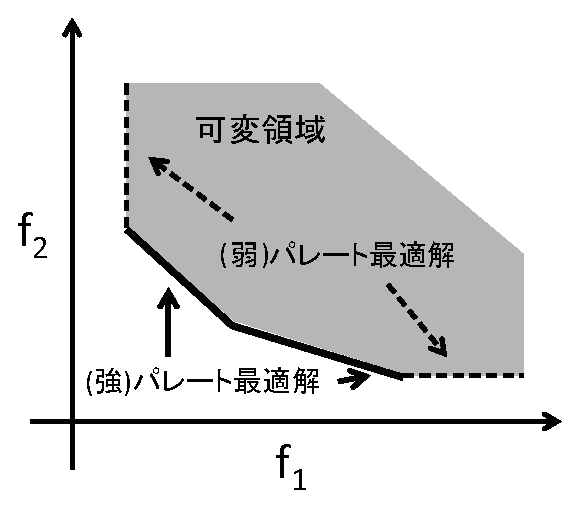
\includegraphics[width=0.5\linewidth]{../figures/pareto.eps}
\end{center}
\caption{パレート最適解の例}
\label{pareto_opt}
\end{figure}

\section{進化的多目的最適化アルゴリズム}
\quad 多目的最適化問題を解く場合,パレート最適解集合が求められることが望ましい.
そこで,多点探索かつ関数の勾配情報を必要としない進化計算を用いてパレート最適解集合を求める方法が提案されている.
進化計算とは,自然界における生物の進化を模倣した計算手法の総称であり,特に多目的最適化に焦点を当てた手法は進化的多目的最適化アルゴリズム(Evolutionary Multiobjective Optimization Algorithms, EMOAs)と呼称される.
EMOAは多点探索を行うことのできる確率的最適化手法であり,多目的最適化問題に対して有効性が示されており,近年注目を集めている.
本研究では,EMOAの中でも遺伝的アルゴリズムを用いて計算を行う.

\section{遺伝的アルゴリズム}
\quad 遺伝的アルゴリズ(Genetic Algorithm, GA)とは,「世代を経るごとに,環境に適さない個体は淘汰され,環境に適した個体同士が生存繁殖することで,より最適な個体となる」という自然界のプロせずから着想を得た最適化アルゴリズムのことである.
実際のアルゴリズムでは,個体集合に遺伝的操作(交叉・突然変異等)を加えることにより,確率的に近似最適解を求めている.
\Figref{GAflow}にアルゴリズムのフローチャートを示す.

\vspace{0.3in}
\begin{figure}[htbp]
\begin{center}
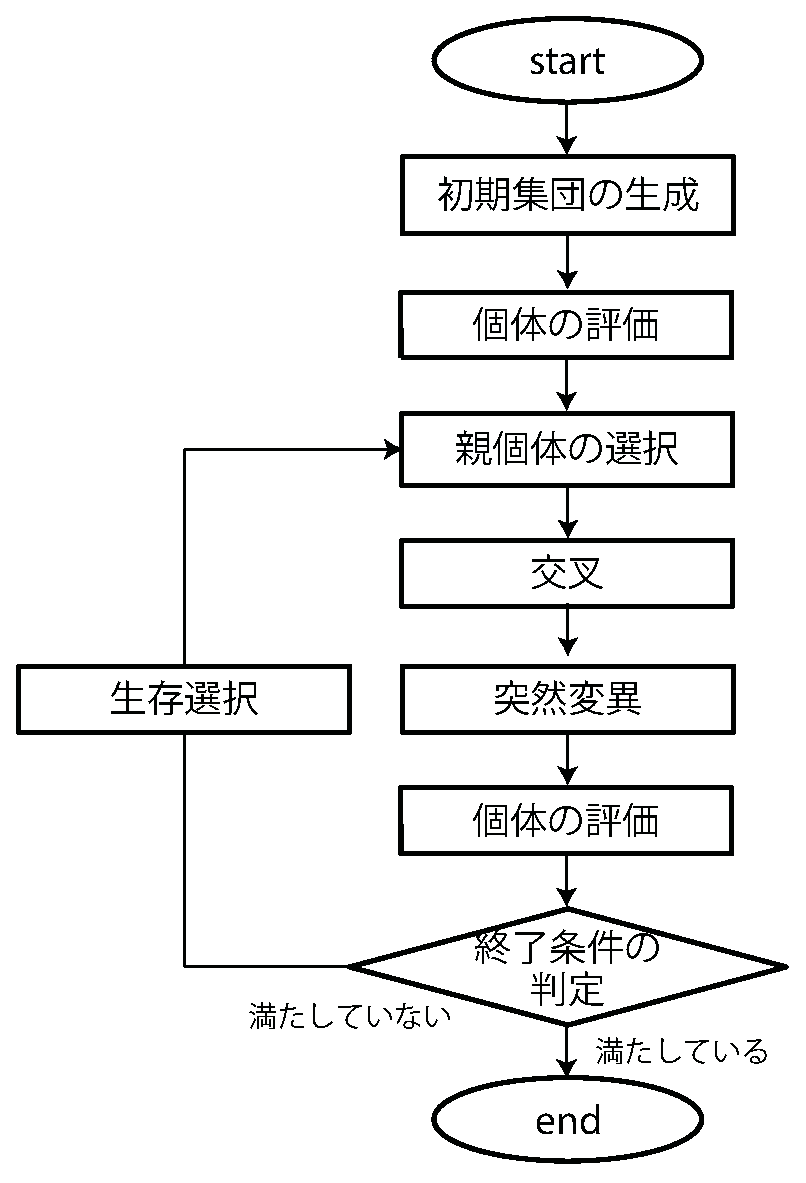
\includegraphics[width=0.6\linewidth]{../figures/flowchart.eps}
\end{center}
\caption{遺伝的アルゴリズム(GA)のフローチャート}
\label{GAflow}
\end{figure}
\afterpage{\clearpage}

\begin{description}
\item[初期集団の生成]\mbox{}\\
「初期集団の生成」では,設定された数(集団サイズ)の個体(解)をランダムに生成する.
ここで生成された個体を初期集団と呼ぶ.

\item[個体の評価]\mbox{}\\
「個体の評価」は,個体集団の中で,どの個体が優れているかを評価する操作である.
個体を評価するために,評価値を算出し,適合度を求める.
適合度は,環境にどれだけ適応しているかを判断する値であり,個体の生き残りやすさを定量的に定めている.
また,制約条件に反しているかどうかについてもこのステップで評価する.

\item[親個体の選択]\mbox{}\\
「親個体の選択」では,「個体の評価」で算出された適合度を基に,子個体を生成する親個体を選択する操作である.
適応度の高い個体ほど親個体に選択されやすく,適応度が低い個体ほど,親個体として選択されにくくなる.

\item[交叉]\mbox{}\\
「交叉」では,「親個体の選択」で選ばれた親個体ペアを用いて,子個体を生成する操作である.
この操作は,自然解での生殖を模倣したものであり,子個体は親個体の特徴を受け継ぐ.
両親個体の特徴を受け継ぐことで,次世代の個体の適応度を上げることを目的としている.

\item[突然変異]\mbox{}\\
「突然変異」では,ある確率(突然変異率)で個体にランダムな変化を与える操作である.
この操作により,局所解に陥ってしまうリスクを回避する.

\item[終了条件の判定]\mbox{}\\
「終了条件の判定」では,このアルゴリズムをどれだけ繰り返し行うかの条件を判定する.
例として,ある世代数に達したときに終了させる条件や,ある計算時間に達した場合終了するといった条件がある.

\item[生存選択]\mbox{}\\
「生存選択」では,次世代に生存する個体を選択する.
「個体の評価」で得られた各個体の適合度を基に,次世代で親個体の選択に用いる集合を決定する.
\end{description}

\section{NSGA-II}
\quad NSGA-II\cite{Deb2002Fast}は,2002年にDebらによって提案されたRCGAの一つである.
本研究では,NSGA-IIを用いて数値実験を行っている.

NSGA-IIは,NSGA \cite{Srinivas1994muiltiobjective}の改良版として提案されたアルゴリズムであり,解の優越性に基づいて個体を評価することが特徴である.
また,生存選択の際に用いられるエリート主義の導入や,解の多様性を維持するためのニッチング手法に,混雑距離(Crowding Distance)を用いていることも特徴の一つである.
NSGA-IIの計算の流れを以下に示す.
さらに,NSGA-IIの進化のイメージを\Figref{nsga_ii}に示す.
また,NSGA-IIで用いられる交叉手法SBX(Simulated Binary crossover)と突然変異手法 polynomial mutation,混雑距離については後述する.

\begin{screen}
\noindent(1)$gen=0$として,初期集団$P_{gen}$を生成する(集団サイズをNとする)\\
(2)個体を評価し,優越関係から親個体を選択する\\
(3)交叉と突然変異を用いて個体を更新し,集団$Q_{gen}$を生成する\\
(4)$R_{gen}=P_{gen}+Q_{gen}$を優越関係を用いて個体を評価し,次の世代集合$P_{gen+1}$を生成する\\
\quad(4.1)優越関係を用いて非劣解集合を順に取り出していき,それぞれ$F_1,F_2,\cdots$という小集合を作る\\
\quad(4.2)$|F_1|+|F_2|+\cdots +|F_n| = N$となった場合,$P_{gen+1}=F_1+F_2+\cdots +F_n$とし,(5)に進み,それ以外の場合(4.3)に進む\\
\quad(4.3)$|F_1|+|F_2|+\cdots +|F_n| \geq N$となった場合,混雑距離を用いて,$F_n$内の個体に優先度をつける\\
\quad(4.4)$F_n$内の優先度の高い個体から順に,$N-(|F_1|+|F_2|+\cdots +|F_{n-1}|)$個取り出した個体集合を新たに$F\prime_n$とし,$P_{gen+1}=F_1+F_2+\cdots +F_{n-1}+F\prime_n$とし,(5)に進む\\
(5)$gen=gen+1$\\
(6)(2)〜(5)を終了条件を満たすまで繰り返す
\end{screen}

\vspace{0.2in}
\begin{figure}[htbp]
\begin{center}
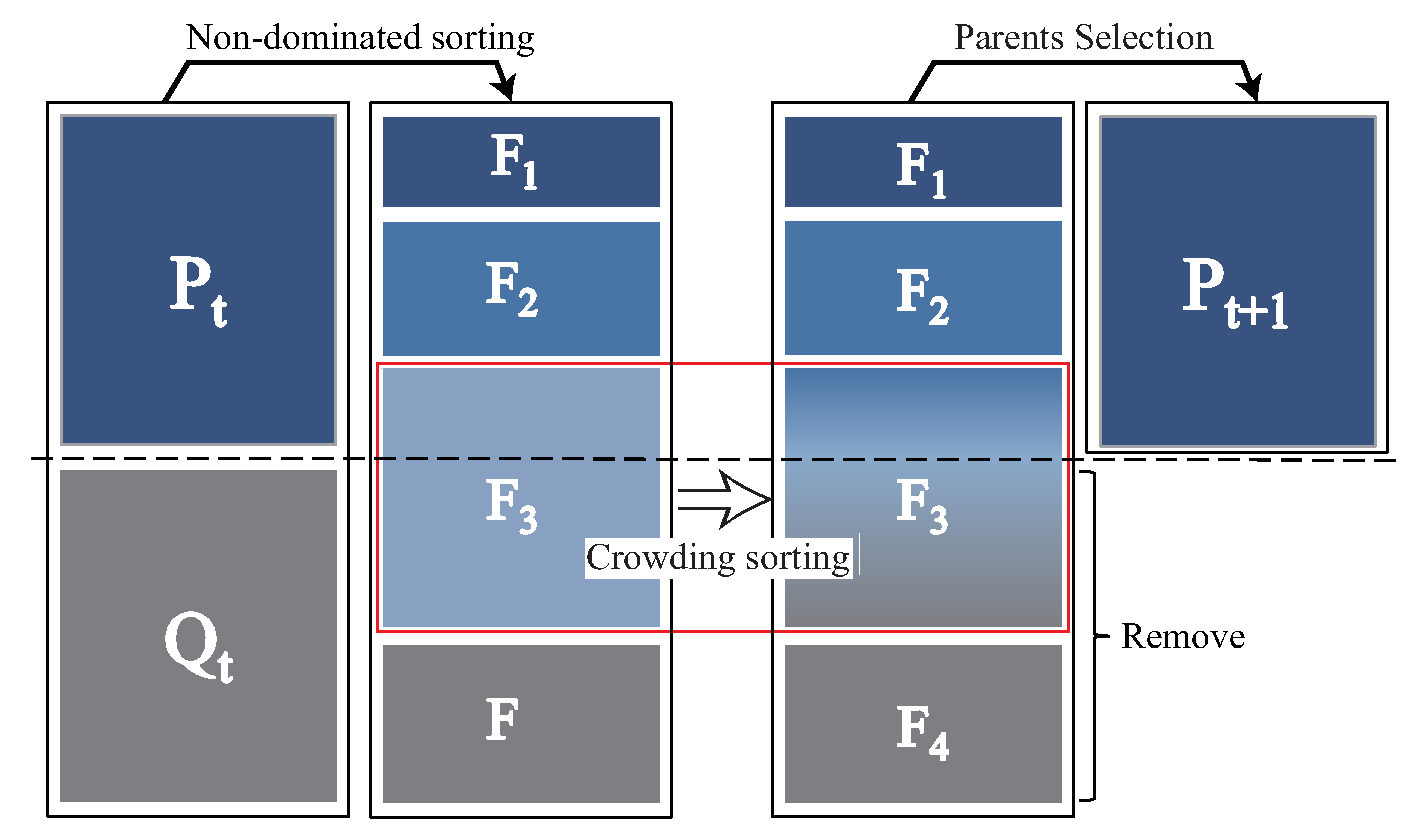
\includegraphics[width=1\linewidth]{../figures/nsga.eps}
\end{center}
\caption{NSGA-IIにおける進化のイメージ図}
\label{nsga_ii}
\end{figure}

\clearpage

\begin{description}

\item[SBX]\mbox{}\\
SBX(Simulated Binary crossover)\cite{Agrawal1995simulated}は,1995年にDebらによって提案された交叉法の一つであり,NSGA-II等多くのGAに採用されている.
SBXを用いた子個体生成の手順を示す.

はじめに,一様乱数uを$0 \leq u \leq 1$の範囲で生成する.
その後,以下で示される確率分布関数と乱数uを用いて,$\beta_q$を算出する.

\begin{equation}
%\begin{align}
\beta_q=\begin{cases}
(2u)^{\frac {1}{\eta_c+1}} & \text{if \ $u<0.5;$} \\
(\frac {1}{2(1-u)})^{\frac {1}{\eta_c+1}} & \text{otherwise.} \\
\end{cases}
%\end{align}
\label{beta}
\end{equation}

ここで,\Eqref{beta}中の$\eta_c$は固有パラメータであり,生成される子個体の分散を制御することができる.
$\eta_c$が大きいほど,子個体は親個体付近に生成されやすく,$\eta_c$が小さいほど,子個体は親個体から遠ざかったところに生成されやすい.

次に,算出した$\beta_q$を用いて,子個体を生成する.
ここで子個体を$x^{(1,t+1)}$,$x^{(2,t+1)}$,親個体を$x^{(1,t)}$,$x^{(2,t)}$とすると,子個体は次の式で算出される.

\begin{subequations}
\begin{align}
x^{(1,t+1)}=0.5[(1+\beta_q)x^{(1,t)}+(1-\beta_q)x^{(2,t)}]\\
x^{(2,t+1)}=0.5[(1-\beta_q)x^{(1,t)}+(1+\beta_q)x^{(2,t)}]
\end{align}
\end{subequations}

\item[Polynomial mutation]\mbox{}\\
polynomial mutation\cite{Deb1996combined}は,1996年にDebらによって提案された突然変異法の一つであり,NSGA-II等多くのGAに用いられている.
polynomial mutationを用いた個体生成の手順を示す.

はじめに,\Eqref{pm_1}に従って親個体$x^t$から$\delta$を算出する.
$x^t_{Upper}$,$x^t_{Lower}$は親個体$x^t$の定義域の最大値,最小値を表している.

\begin{equation}
\delta=\frac{min(x^t_{Upper}-x^t,x^t-x^t_{Lower})}{x^t_{Upper}-x^t_{Lower}}
\label{pm_1}
\end{equation}

次に,一様乱数uを$0 \leq u \leq 1$の範囲で生成し,以下で示される確率分布関数と乱数uを用いて,$\delta_q$を算出する.

\begin{equation}
%\begin{align}
\delta_q=\begin{cases}
[2u+(1-2u)*(1-\delta)^{\eta_m+1}] ^{\frac {1}{\eta_m+1}}-1& \text{if \ $u<0.5;$} \\
1-[2(1-u)+2(u-0.5)*(1-\delta)^{\eta_m+1}] ^{\frac {1}{\eta_m+1}} & \text{otherwise.} \\
\end{cases}
%\end{align}
\label{delta}
\end{equation}

ここで,\Eqref{delta}中の$\eta_m$は固有パラメータであり,生成される子個体の分散を制御することができる.
$\eta_m$が大きいほど,子個体は親個体付近に生成されやすく,$\eta_c$が小さいほど,子個体は親個体から遠ざかったところに生成されやすい.
次に,算出した$\beta_q$を用いて,子個体を生成する.子個体を$x^{t+1}$とすると,子個体は\Eqref{pm_2}で算出される.

\begin{equation}
x^{t+1}=x^t+\delta_q(x^t_{Upper}-x^t_{Lower})
\label{pm_2}
\end{equation}

\item[混雑距離(Crowding Distance)]\mbox{}\\
混雑距離とは,目的関数空間内での個体間の距離を計算するものである.
NSGA-IIでは,混雑距離を算出し,生き残る個体の優先度を決めることで,個体が偏って生成されてしまうのを防ぐ,ニッチング法に用いられている.
個体$d_i$の混雑距離は\Eqref{cd_eq1},(\ref{cd_eq2})で算出される.
なお,目的関数の数を$m$,$S$を非劣解集合,$|S|$を非劣解の数,$f_k$を第k目的関数とする.
また,i番目の個体の混雑距離のイメージを\Figref{cd}に示す.

\begin{equation}
d_1=d_{|S|}=\infty \\
\label{cd_eq1}
\end{equation}
\begin{equation}
d_i=\sum_{k=1}^m \sum_{i=2}^{|S|-1} |f_k(i+1)-f_k(i-1)|\\
\label{cd_eq2}
\end{equation}

\begin{figure}[htbp]
\begin{center}
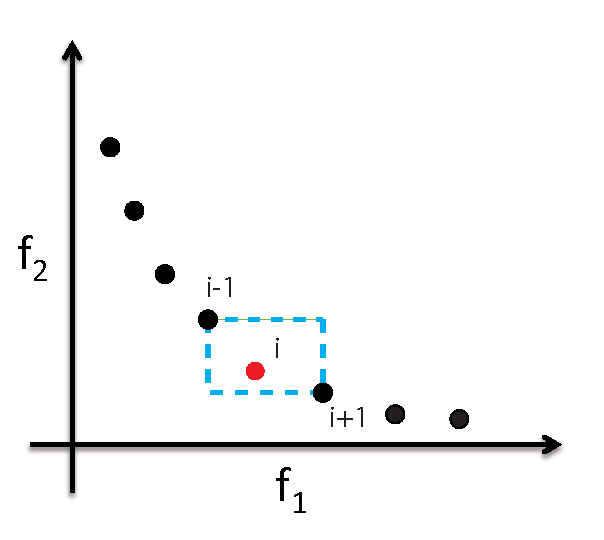
\includegraphics[width=0.3\linewidth]{../figures/crowding.eps}
\end{center}
\setlength{\abovecaptionskip}{-5mm}
\setlength{\belowcaptionskip}{0mm}
\caption{混雑距離のイメージ図}
\label{cd}
\end{figure}

\Figref{cd}のように隣り合う個体を用いて,i番目の個体の周りに骨格を取る.
その後,骨格の片側の2辺を足し合わせた値が,i番目の個体の混雑距離となる.

混雑距離を求めることで,各個体の疎密度が算出される.
したがって,混雑距離によってソートを行うことで,疎な解が生存しやすくなるため,解の多様性を維持する機構として用いられている.

\end{description}

\section{MOEA/D}
\quad MOEA/D (Multi-objective Evolutionary Algorithm Based on Decomposition)\cite{Zhang2007MOEAD}は2007年にZhangらによって提案されたRCGAの一つである.
本研究においても,数値実験に使用している.

MOEA/Dでは探索空間上に重みベクトルを均一の間隔で分布させ,それらの重みベクトルとスカラー適応度関数を用いて,多目的最適化問題をベクトル毎の単一目的最適化の部分問題へと帰着させる.
その後,各重みベクトルに対し,ユークリッド距離の近いベクトルを近傍とし,近傍内において遺伝的操作(交叉や突然変異)を行う.
また,MOEA/Dでは最適化に用いる個体群とは別に,計算中に得られた非劣解群をアーカイブとして保持する機構を持つ.

MOEA/Dの計算の流れを以下に示す.

\begin{description}
\item[Step 1 : 初期化]\mbox{}\\
\vspace{-0.5in}
	\begin{description}
	\item[1.1 : 重みベクトル生成]\mbox{}\\
	探索に用いる$N$個の重みベクトル${\bm \lambda}$を\Eqref{omomi}により生成する.
	\begin{eqnarray}
	\left.
	\begin{array}{rcl}
	{\bm \lambda} & = & (\lambda_1, \lambda_2, \cdots, \lambda_k)\\
	\sum_{i=1}^{k} \lambda_i & = & 1\\
	N & = & {}_{H+k-1}C_{k-1}\\
	where & \lambda_i & \in \left\{ \cfrac{0}{H}, \cfrac{1}{H}, \cdots, \cfrac{H}{H} \right\}
	\end{array}
	\right\}
	\label{omomi}
	\end{eqnarray}
	
	ここで,$k$は目的関数の数,$H$は分割数を表す.
	
%	\vspace{-0.1in}
	
	\item[1.2 : 近傍ベクトル生成]\mbox{}\\
	1.1で作成した各ベクトル間のユークリッド距離を計算し,各ベクトル$\bm \lambda^i$に最も近い$T$個のベクトル$\bm \lambda^{i_1}, \cdots, \bm \lambda^{i_T}$を$\lambda^i$の近傍とする.
%	\vspace{-0.1in}
	
	\item[1.3 : 初期個体群生成]\mbox{}\\
	ベクトルの総数$N$個と等しい数の初期個体をランダムに生成し,1つのベクトルに対し1つの個体を対応させる.
%	\vspace{-0.1in}
	
	\item[1.4 : 参照点更新]\mbox{}\\
	参照点$\bm z^*$の更新を\Eqref{sansyou}によって行う.
	
	\begin{eqnarray}
	\left.
	\begin{array}{rcl}
	{\bm z^*} & = & (z_1^*, z_2^*, \cdots, z_k^*)\\
	z^*_j & = & \max \left\{ f_j (\bm x) | \bm x \in \bm X \right\}
	\end{array}
	\right\}
	\label{sansyou}
	\end{eqnarray}
	
	ここで,$f_j (\bm x)$は個体$\bm x$の$j$番目の目的関数,$\bm X$は設計変数空間内での実行可能領域を表す.
	
	\vspace{-0.1in}

	\end{description}
\item[Step 2 : 遺伝的操作]\mbox{}\\
\vspace{-0.5in}
	\begin{description}
	\item[2.1 : 親個体選択]\mbox{}\\
	ベクトル$\bm \lambda^i$の近傍ないからランダムに2つの個体を選択する.
%	\vspace{-0.1in}
	
	\item[2.2 : 子個体生成]\mbox{}\\
	2.1で選択された親個体から交叉(SBX)と突然変異(polynomial mutation)を行い子個体を生成する.
%	\vspace{-0.1in}
	
	\item[2.3 : 参照点更新]\mbox{}\\
	\Eqref{sansyou}を用いて参照点を更新する.
%	\vspace{-0.1in}
	
	\item[2.4 : 近傍解更新]\mbox{}\\
	2.2で生成された子個体と$\bm \lambda^i$近傍内のベクトルに対応する個体をスカラー適応度関数を用いて比較し更新する.
	スカラー適応度関数は主に Tchebycheff Approach と Weighted Sum Approach がある.
	本研究で用いるTchecycheff Approach を以下に示す.
	
	\begin{eqnarray}
	\left.
	\begin{array}{rccl}
	minimize & g^{te} (\bm x|\bm \lambda , \bm z^*)& =& \mymax_{1 \leq i \leq m} \{ \lambda_i|f_i (\bm x) - z^*_i| \}\\
	sub.to & x \in X &  &  \\
	where & z^* & = & (z_1^*, \cdots, z^*_k)^T
	\end{array}
	\right\}
	\label{sansyou}
	\end{eqnarray}
	
	
%	\vspace{-0.1in}
	
	\item[2.5 : アーカイブ更新]\mbox{}\\
	非劣解となった子個体をアーカイブに追加し,アーカイブ内の劣解を削除する.
	\vspace{-0.1in}
	
	\end{description}
\item[Step 3 : 終了判定]\mbox{}\\
%\vspace{-0.5in}

\end{description}


上述のアルゴリズムにおいて,Step2の操作を終了判定を満たすまで繰り返すことで解の探索を行う.


\section{解の評価指標について}
\quad 本項では,本研究で用いた多目的最適化における解の評価指標について述べる.

\subsection{GD}
Generational Distance (GD)\cite{Deb2002Fast} とは解の収束性を評価する際に用いる評価指標である.
GDは,得られた非劣解集合の各点から真のパレートフロントまでの最短距離の平均値を算出する指標である.
値が小さいほど収束性が良いことを示し,0が最小値となる.
GDは\Eqref{gd_formulation}で定式化される.

\begin{eqnarray}
\begin{array}{rcl}
GD(\bm S,\bm P)&=&\cfrac{\left( \sum^{|\bm S|}_{i=1} d_i^2 \right) ^ {1/2}}{|\bm S|}\\
d_i & = & \min_{\vec p \in \bm P} || F(\vec{s_i}) - F(\vec p) ||
\label{gd_formulation}
\end{array}
\end{eqnarray}

$\bm S$は得られた非劣解集合,$\bm P$は理論上のパレートフロントの点集合を示す.
また,$d_i$は$\bm S$の各点から$\bm P$の最短距離となる点への距離を示し,$|\bm S|$は$S$の点数を示す.


\subsection{IGD}
Inverted Generational Distance (IGD)\cite{Zhou2006combining} とは解の収束性と解の多様性を同時に評価できる総合評価指標である.
IGDは,真のパレートフロントの各点から得られた非劣解集合までの最短距離の平均値を算出する指標である.
値が小さいほど収束性と多様性が良いことを示し,0が最小値となる.
IGDは\Eqref{igd_formulation}で定式化される.

\begin{eqnarray}
\begin{array}{rcl}
IGD(\bm P,\bm S)&=&\cfrac{\left( \sum^{|\bm P|}_{i=1} d_i^2 \right) ^ {1/2}}{|\bm P|}\\
d_i & = & \min_{\vec s \in \bm S} || F(\vec{p_i}) - F(\vec s) ||
\label{igd_formulation}
\end{array}
\end{eqnarray}

$\bm S$は得られた非劣解集合,$\bm P$は理論上のパレートフロントの点集合を示す.
また,$d_i$は$\bm P$の各点から$\bm S$の最短距離となる点への距離を示し,$|\bm P|$は$P$の点数を示す.


\end{document}